\documentclass[a4paper,titlepage,11pt]{report}
\usepackage{frontespizio}
\usepackage{geometry}
\usepackage{lmodern}
\usepackage[cache=false]{minted}
\usemintedstyle{friendly}
\usepackage[english]{babel}
\usepackage[dvipsnames]{xcolor}
\usepackage{imakeidx}[column=1, title=Indice, intoc]
\usepackage{subfig}
\usepackage{graphicx}
\definecolor{blu_pant}{RGB}{0, 64, 122}
\geometry{bmargin=3.5cm, rmargin=2.5cm, lmargin=2.5cm, footnotesep=1cm}
\usepackage{setspace}
\setstretch{1.5}
\makeindex[columns=1, title=Indice, intoc]
\begin{document}
{\fontfamily{lmr}\selectfont
\begin{frontespizio}
\Istituzione{University of Pisa}
\Divisione{Department of Computer Science}
\Scuola{Master's Degree of Computer Science \\(Artificial Intelligence)}
\Piede{Academic year 2022/2023}
\Titoletto{Artificial Intelligence Fundamentals}
\Titolo{\textcolor{black}{Football-betting Detection System}}
\NCandidato{Project made by}
\Rientro{2.5cm}
\Candidato{Andrea Tufo}
\end{frontespizio}



\pagebreak



\tableofcontents



\chapter{
Introduction\index{Introduction}}
In this document all the specifications of the project can be found, including not only theorical explainations, but also instances, useful to enucleate the code.\\
The first chapter is going to introduce how the projects actually works, and why it would be useful for football and more in general for sport. This section is also important to figure out the idea behind the algorithm and how all the development has been organized.\\
All the main difficulties that I faced during the development and all the most important issues that my algorithm has, are listed in the end of this document, where are explained some possible solutions too, in order to solve them and improve the algorithm.

\section{
Sport-betting}
The Sport-betting phenomenon is still nowadays one of the worse side of the sports. It hurts two sports above all: tennis and football. The former because, since there are very few actors involved in the game (for example only two players), it's very easy bribing one of them or both of them and change the flow of events.\\
The latter because football moves a huge amount of money, thus it's very easy to became millsionaire corrupting one or two match per season.\\
The \textit{modus operandi} is always the same, "bribe and earn", so "sport criminals" used to corrupt players, who have the role to make the match ends as agreed, then criminals will be able to bet and so collect thier money.


\chapter{
Implementation\index{Implementation}}
The main goal was to develop a system that rely and analyze football matches data, showing a percentage of "possible unfair match". The basic idea was to retrive some parameters and values from raw filtered data, collect them, and then looking for some anomalies. In the code has been used as case of study the 2012/2013 season of Serie A, so every match that belongs to the regular season. In my case there is one important metric, which is called \textit{"OPI" (Offensive Potential Index)} and has the role to mesure how a team has been dangerous and offensive during a match, so this value is computed for each football team. 

formula OPIOPI

\section{
Dataset}
During the first phase, after the inital study of the phenomenon, i had to select a reliable dataset from the Internet, so in the project my choise was to pick up a dataset found on kaggle, which contains six seasons data of five championships. Of course these raw datas were no ready to be used for my program, thus, filtering them and select only the needed ones was the first operation that I implemented. The dataset is made up two csv files, one "ginf.csv" that contains all the matches (with home and away team name, goals, stadium, season, league), while the second one called "events.csv", contains all the events per match and so fouls, shots, ball possesion losses, corners, penalties and more. These two files are connected like in DBs, every match in "ginf.csv"  has an unique id, that identifies it in the other file.\\
All the first effort was focused on filtering all the data of the 2012/2013 italian season, collecting 380 matches, with all statistics and events. 

\subsection{
Events file}
The events file has three main columns: the event\_type, which throught an index give us the information on what type of event has happened (for example 1 for shot), than there is the event\_team that contains the name of the team that generates that specific event and finally the location column which indicates the position of the events throught a sort of field mapping.\\
Of course there are many more attributes that are very important like the final outcome of the shot (goal, post hit, blocked not in target), or the description of the event but we will focuse only on this three parameters because are the most used in the code.

\section{
Filtering}
The filtering phase has been very hard to implement because only during coding the algorithm logic I figured out step by step what kind of data my program needed. So the main operation could be divided into two parts: the first one in which I filter the useless matches, selecting only the matches on which I was intrested to work on, while during the second part my goal was to select only the correct datas from the events file. The data selected per single match were: the goals scored by home and away team, the victory, draw and loose probability, the number of shots, the locations of evry single shot excluding the shots that had as outcome "goal scored".\\
During the first run of the algorithm a "filtered\_dataset.csv" file is generated, it contains all the data filtered in order to avoid to fetch and to filter more times the data from the biggest file, because it takes too much time to do it. 

\subsection{
Offensive Potential Index}
Pratically in my program I worked on only one json object, which contains all the data filtered and makes more easy get all the metrics from every single match. The biggest challenge for me was to find out some parameters that would have highlighted how much offensive a team has been during a match in average. And my idea was to analyze every match looking at the shots made by a team and their locations. So for all matches I group the two arrays of shots locations (one for home team and one for away team) into three group, each of this group has a weight that refers to the possibility to score, thus, fisrt group has weight one, so very low dangerous shot, the second one has weight two, and the third one has three as weight, and so high chances to score.\\
Then I caluclated the cardinality of these three sets and after this I computed the \textit{OPI} summing up the cardinalities timed for the weight of the group on which they belong to.


\chapter{
Final results and HMM application}
In order to apply this model, a transition model and a sensor model are needed. The transition model is made up starting from two states, that are: less than 2 goals scored state and 2 or more than two goals scored by a team. So the algorithm calculates, taking as input a random team as sample, how many times in average a team goes in each state from a starting state.\\
The sensor model is based on the OPI index, so the two evidences are: low OPI, and high OPI. Basically the system calculates the mean and the variation of all the team's OPIs taking all the matches OPI. Throught this two values I found a good interval in order to determine a low OPI situation (actual OPI less or equals than the interval) or a high OPI situation (actual OPI more than the interval). Accordingly, as what happens  for the transition models the program calculates for every state how many times in average we are in low and high OPI condition.\\
interval formula
In the output the algorithm shows the target match the final result and the probability that we are into a fixed match. Furthermore the algorithm shows some previous and next matches of both teams, with result and probability too. In my specific case the fixed match is Pescara 2 - Siena 3, and these are the results:

\begin{tabular}{c c}
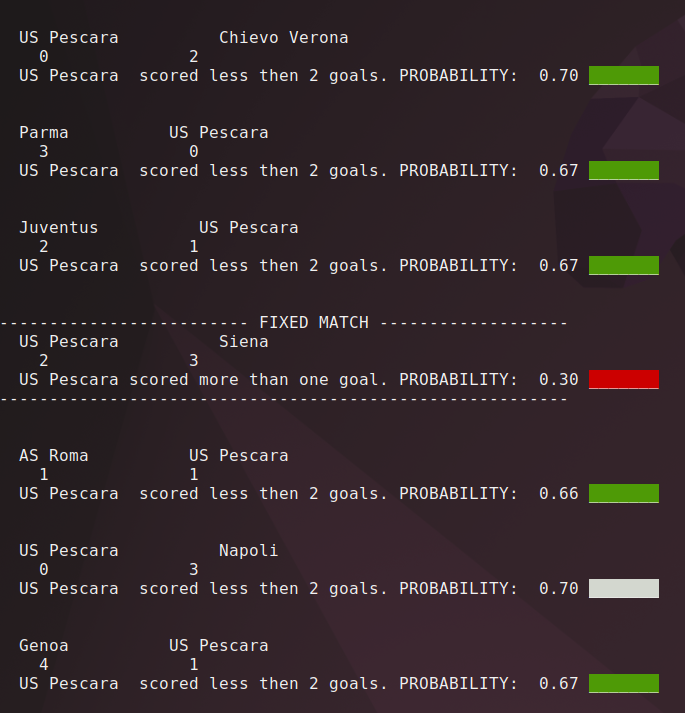
\includegraphics[scale=0.3]{results1.png} &
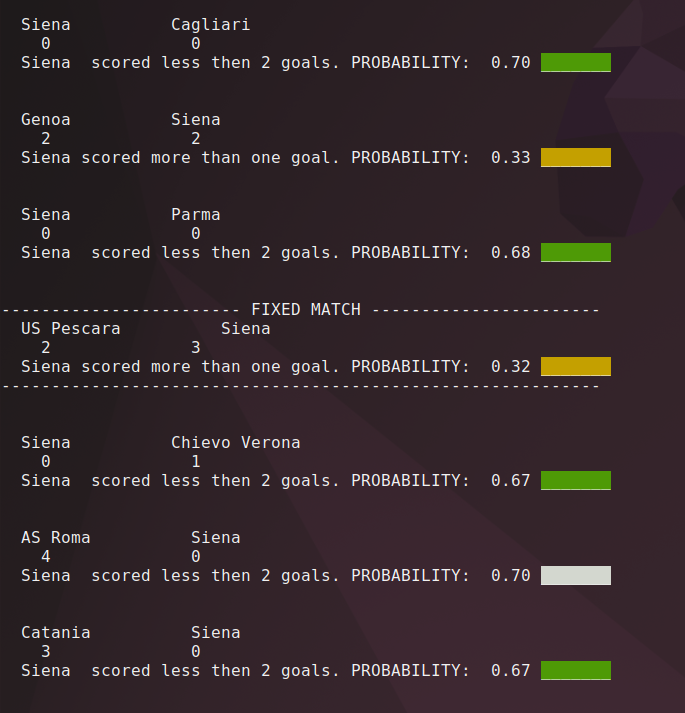
\includegraphics[scale=0.3]{results2.png}
\end{tabular}
\end{document}